%%%%%%%%%%%%%%%%%%%%%%%%%%%%%%%%
%%%%%%%%%%%%%%%%%%%%%%%%%%%%%%%%
%%%%%%%%%%%%%%%%%%%%%%%%%%%%%%%%

\section{CHWP AR requirements}
\label{sec:sapphire_ar_coating_requirements}

Requirements on the 

As is somewhat evident from the the table in Figure~\ref{fig:one_two_three_layer_ar_coating_optimization}, the optimal for each AR layer, no matter the total number of layers, is close to $d_{\lambda / 4}$ for the AR band's central frequency of $\approx$~122~GHz.\footnote{There are $\sim$~few percent deviations in the three-layer coating that trade bandwidth for reflection suppression in PB-2b's fixed bandwidth.}. Therefore, a useful relation when estimating the optimal thickness of each layer in the AR coating is to use Equation~\ref{eq:lambda_over_four_thickness}, where $\lambda_{0}$ is the AR band's central frequency. 

\begin{figure}
    \centering
    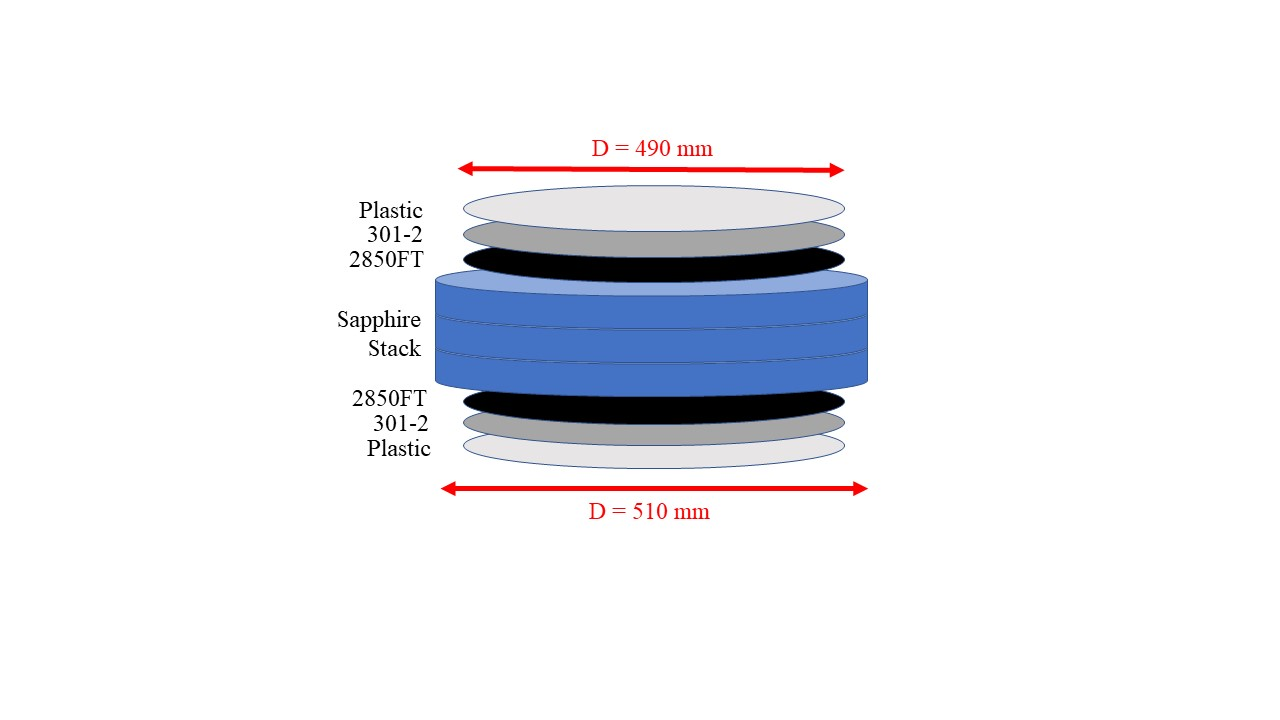
\includegraphics[width=0.98\linewidth]{ARCoating/Figures/sapphire_ar_stack_cartoon.jpg}
    \caption[Cartoon of the a sapphire stack with an epoxy+plastic anti-reflection coating]{Cartoon of the a sapphire stack with an epoxy+plastic anti-reflection coating. The bottom AR layer is molded directly onto the sapphire surface, which is primed with an adhesion promoter. The top AR layer is glued onto the machined bottom layer using EpoTek 301-2 optical epoxy.}
    \label{fig:ar_cartoon}
\end{figure}

\begin{figure}
    \subfloat[\label{fig:epoxy_duroid_meas:a}]{
        \raisebox{1cm}{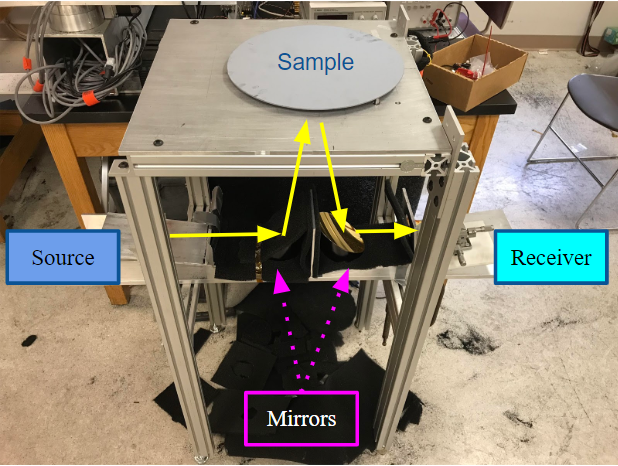
\includegraphics[width=0.48\linewidth]{ARCoating/Figures/grace_reflectometry_setup.png}}
    }
    \subfloat[\label{fig:epoxy_duroid_meas:b}]{
        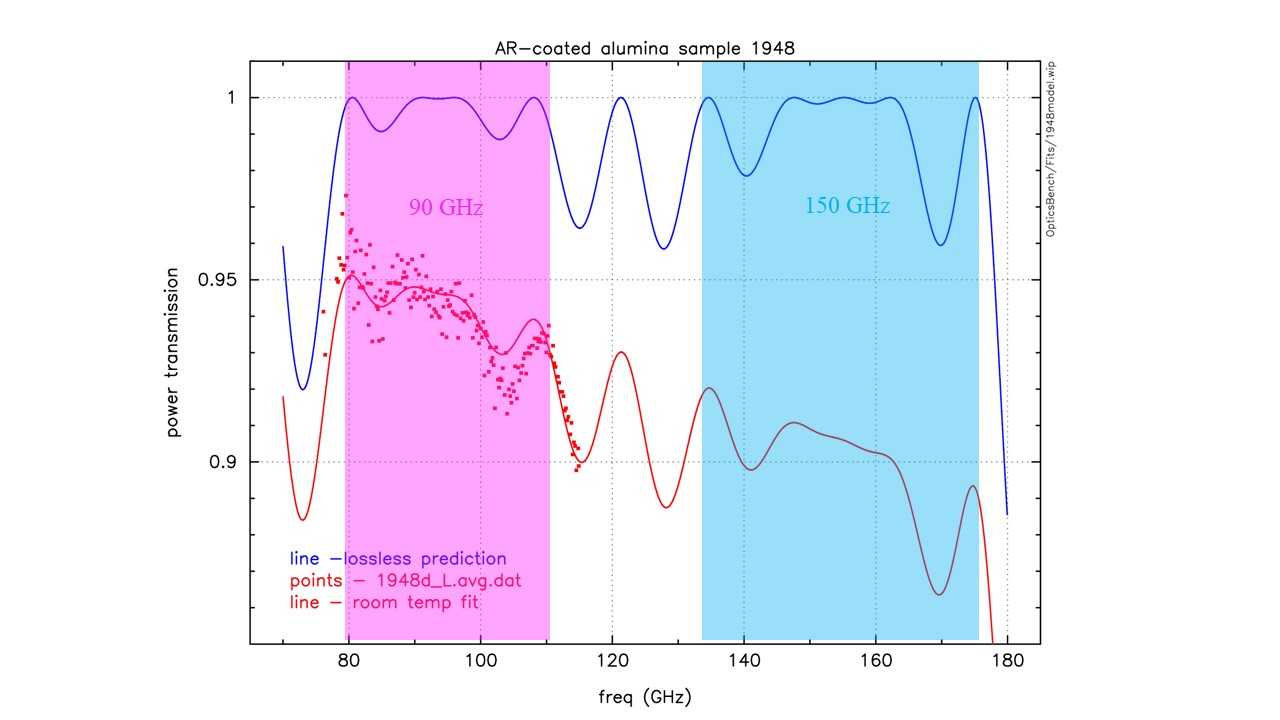
\includegraphics[width=0.48\linewidth]{ARCoating/Figures/duroid_epoxy_ar_measurement.jpg}
    }
    \caption[Measurement of the epoxy + Duroid AR coating at both room and cryogenic temperatures]{Measurement of the epoxy + Duroid AR coating at both room and cryogenic temperatures. \ref{fig:epoxy_duroid_meas:a} shows the Chicago reflectometry setup used to measure the AR coatings. A pyramidial horn generates a coherent polarized beam which is collimated by a parabolic input mirror, reflected off of the sample, collimated by an identical output parabolic mirror, and collected by an identical pyramidal horn. The output signal is then mixed with the input tone to measure the output phase and amplitude. \ref{fig:epoxy_duroid_meas:b} shows the reflection of the sample at both warm and cold temperatures. TODO: THIS FIGURE NEEDS TO BE UPDATED WHEN WE HAVE ONE THAT IS PUBLISHABLE}
    \label{fig:epoxy_duroid_meas}
\end{figure}

\begin{figure}
    \subfloat[\label{fig:ar_layers_fts:a}]{
        \raisebox{1cm}{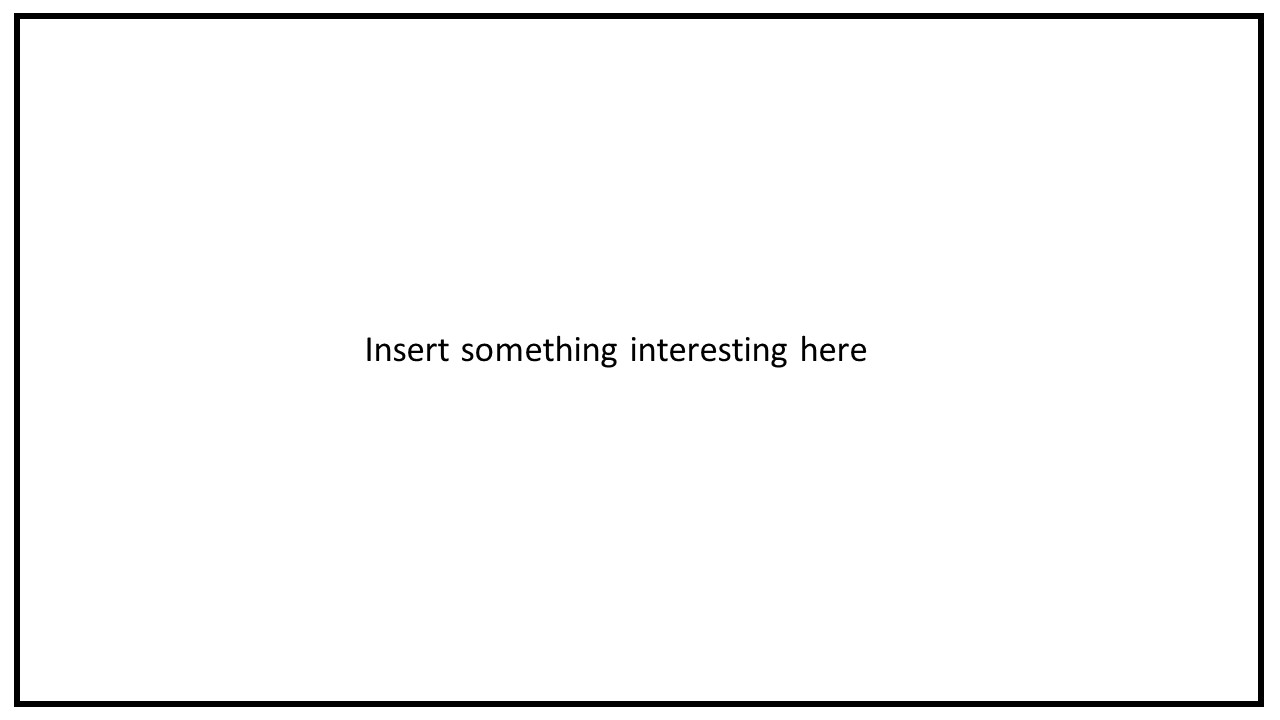
\includegraphics[width=0.48\linewidth]{Other/empty.jpg}}
    }
    \subfloat[\label{fig:ar_layers_fts:b}]{
        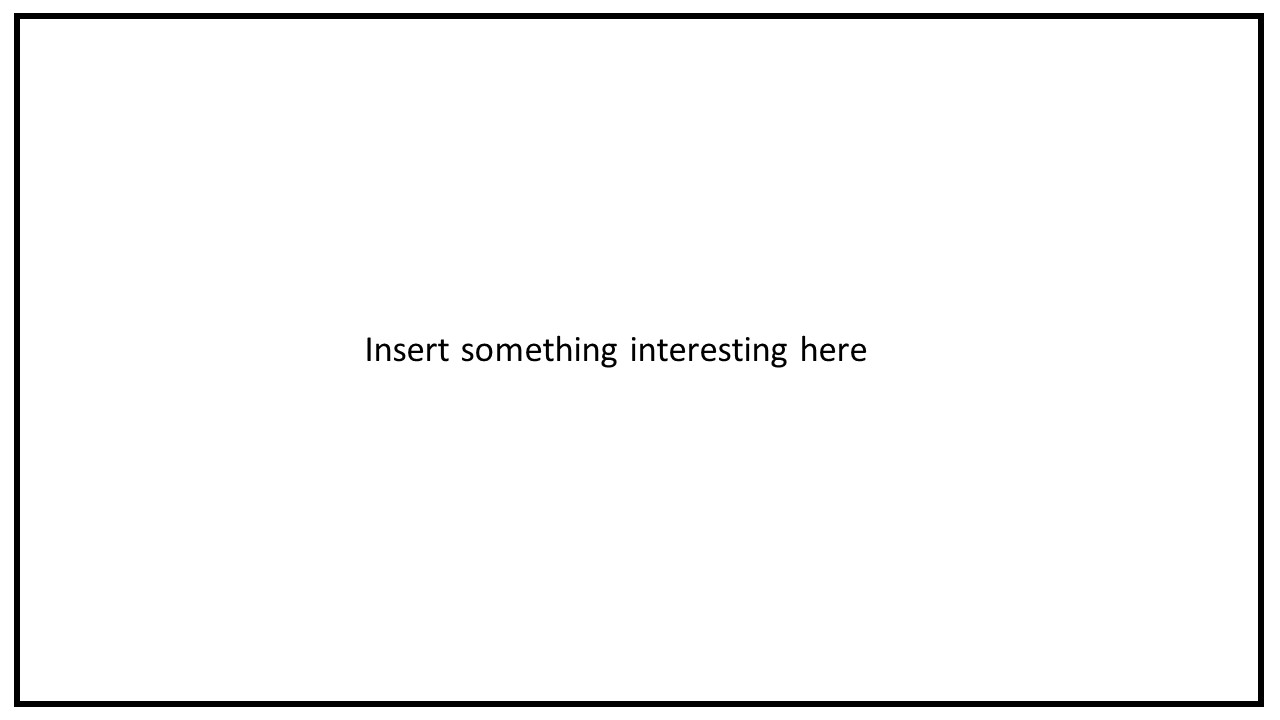
\includegraphics[width=0.48\linewidth]{Other/empty.jpg}
    }
    \caption[Room temperature and cryogenic transmission measurements of Stycast 2850FT, Duroid 5880LZ, and Vespel SF-0940]{Room temperature and cryogenic transmission measurements of Stycast 2850FT, Duroid 5880LZ, and Vespel SF-0940. These figures will hopefully be provided by Makoto}
    \label{fig:ar_layers}
\end{figure}

Unlike with the PB-2a WHWP whose AR coating is described in Section~\ref{sec:pb2a_whwp_ar_coating}, t

There are different process parameters to sandblasting, including grit size, spray pressure, and the spray nozzle's distance to the sapphire surface. 